\chapter{关于泛化的VC理论}

泛化,指的是学习到的模型对于未知数据的预测能力. 半世纪前,Vapnik-Chervonenkis理论(简称VC理论)被提出,尝试从数学角度定量地刻画了所谓泛化能力. 值得一提,现如今VC理论被指出并不能完整地刻画“泛化”,即仍有该理论未囊括的额外因素,但其思想是重要且值得介绍的. 

\section{机器学习的数学描述}

首先介绍一个基本概念:
\begin{definition} (模型,函数类,假设空间)
    给定输入空间$\mathcal{X}$和输出空间$\mathcal{Y}$,那么由其确定的模型(Model),函数类(Function Class)或假设空间(Hypothesis Space)(这三者是同义词)为 
    \[
    \ca{F} = \{f:\ca{X} \ra \ca{Y}\}
    \]
\end{definition}

例如:全体二次函数、线性函数或CNN都可以叫做模型. 

\medskip
现在考虑一个简单的有监督学习的模型,有数据集$(x_1, y_1), \dots, (x_n, y_n)$,其中$x_i \in \mathcal{X}, y_i \in \mathcal{Y}$,所有数据i.i.d.且服从$D_{X,Y}$. 我们称每个$x_i$为\textbf{实例}(instance),每个$y_i$为\textbf{标签}(label).

有了数据,便要进行训练. 这里便可以看出假设空间的重要性了,我们总是在假设空间中进行学习,而非天马行空毫无约束. 记假设空间为$\ca{F}$,现在我们要选择$\hat f \in \ca F$使得其在数据集$\{(x_i, y_i)\}_{i=1}^n$上有一个较小的损失(loss)或误差(error).

那么如何评判$\hat f$的好坏?一个直观上的评估就是在$D_{X,Y}$上的错误率. 

\begin{definition}(训练误差) 
    有监督学习的情况下,对于数据集$\{(x_i, y_i)\}_{i=1}^n$和假设$\hat f$,训练误差(Training Error)为
    \[
    \dfrac{1}{n} \sum_{i=1}^n \mathbb{I}[y_i \neq \hat f(x_i)]
    \]
\end{definition}

\begin{definition}(泛化误差) 
    有监督学习的情况下,设数据$(X, Y)$服从分布$D_{X,Y}$,对于假设$\hat f$,泛化误差(Generalization Error)为
    \[
    \Pr_{(X, Y) \sim D_{X,Y}}\left[
        Y \neq \hat f(X)
    \right]
    \]
\end{definition}

自然地,我们可以得到泛化差距
\begin{definition}
    承之前所有记号,$\hat f$的泛化差距(Generalization Gap)为 
    \[
    \Pr_{(X, Y) \sim D_{X,Y}}\left[
        Y \neq \hat f(X)
    \right] - \dfrac{1}{n} \sum_{i=1}^n \mathbb{I}[y_i \neq \hat f(x_i)]
    \]
\end{definition}

如果我们记$Z_i := \mathbb{I}[y_i \neq \hat f(x_i)]$以及$Z := \mathbb{I}[Y \neq \hat f(X)]$. 那么泛化差距就可以写成$\E[Z] - \frac{1}{n} \sum_i Z_i$. 由于每个$Z_i$和$Z$都服从某个Bernoulli分布,这看起来似乎就像是我们在前一章集中不等式当中描述的样子. 那么泛化差距应该随着数据集的大小$n$的增长指数级收敛至$0$. 也就意味着泛化永远成立?但事实并非如此,这个$\hat f$是由$\ca D := \{(x_i, y_i)\}_{i=1}^n$确定的,因此$\hat f$依赖于$\ca D$. 此时$Z_1, \dots, Z_n$根本不独立,甚至某些程度上正相关,因此不能应用Chernoff界. (另外,回忆一下\textbf{1.3节}中负相关才能放缩,正相关时不一定成立)

接下来探讨何时泛化差距会比较小. 

\section{有限假设空间下的结果}

先来考虑假设空间$\ca F$是有限集的情况($|\ca F| < \infty$). 请注意该情况是过于简化的,因为线性模型都是无穷集. 记$\ca F = \{f_1, \dots, f_{|\ca F|}\}$,考虑算法最差的情况下对于任意$\varepsilon > 0$

\begin{align*}
    & \Pr_{\text{worst case}} \left[
        \Pr_{(X, Y) \sim D_{X,Y}} \left[
            Y \neq \hat f (X)
        \right] - \dfrac{1}{n} \sum_{i=1}^n \mathbb{I}[y_i \neq \hat f(x_i)] \ge \varepsilon
    \right] \\
    \le & 
    \sum_{j=1}^{|\ca F|} \Pr\left[
        \Pr_{(X, Y) \sim D_{X,Y}} \left[
            Y \neq f_j (X)
        \right] - \dfrac{1}{n} \sum_{i=1}^n \mathbb{I}[y_i \neq f_j(x_i)] \ge \varepsilon
    \right] \\ 
    \le & |\ca F| \cdot e^{-2n\varepsilon^2}
\end{align*}

可以看到$\ca F$有限时泛化误差几乎必然随着$n$增大而收敛到一个较小的值. 但这样的分析不足以支撑$|\ca F|$是无穷的情况,这就需要使用VC理论了.

\section{无穷假设空间下的放缩}
现在考虑$|\ca F| = \infty$的情况,依旧有
\begin{align}
        & \Pr_{\text{worst case}} \left[
        \Pr_{(X, Y) \sim D_{X,Y}} \left[
            Y \neq \hat f (X)
        \right] - \dfrac{1}{n} \sum_{i=1}^n \mathbb{I}[y_i \neq \hat f(x_i)] \ge \varepsilon
    \right] \\ \label{eq:generalization-err-ineq}
    & \le \Pr\left[
        \sup_{f\in \ca F}\Pr_{(X, Y) \sim D_{X,Y}} \left[
            Y \neq f (X)
        \right] - \dfrac{1}{n} \sum_{i=1}^n \mathbb{I}[y_i \neq f(x_i)] \ge \varepsilon
    \right]
\end{align}

我们想区分假设空间的大小关系(需要一个比基数更好的度量方式),例如五次函数类应该比线性函数类要大. 逐步来讨论,先证明一个引理 

\begin{lemma}
    设$X, X_1, \dots, X_n, X_{n+1}, \dots, X_{2n}$是i.i.d的随机变量且服从Bernoulli分布. 记$\nu_1 = \frac{1}{n} \sum\limits_{i=1}^{n} X_i, \nu_2 = \frac 1n \sum\limits_{i=n+1}^{2n} X_i$,并设$\E[X]=p$. 若$n > \varepsilon^{-2} \ln 2$,则
    \[
    \frac 12 \Pr\Big[
        \abs{\nu_1-p} \ge 2\varepsilon
    \Big] \leq 
    \Pr\Big[
        \abs{\nu_1 - \nu_2} \ge \varepsilon
    \Big] \leq 
    2 \Pr\left[
         \abs{\nu_1-p} \ge \frac{\varepsilon}2
    \right]
    \]
\end{lemma}
\begin{proof}
    我们分两部分证明.

    \begin{enumerate}
        \item[\Circled{1}]右半式较为简单,若$\abs{\nu_1 - \nu_2} \ge\varepsilon$,那么必然有$\abs{\nu_1-p} \ge \frac\varepsilon 2$或$\abs{\nu_2-p} \ge \frac\varepsilon 2$,而后面二者概率相等,故
    \[
    \Pr\Big[
        \abs{\nu_1 - \nu_2} \ge \varepsilon
    \Big] \leq 
    2 \Pr\left[
         \abs{\nu_1-p} \ge \frac{\varepsilon}2
    \right]
    \]
        \item[\Circled{2}] 再来看左半式,由于$\nu_1$和$\nu_2$是两个独立的随机变量,所以 
        \begin{align*}
            \Pr \big[
                \abs{\nu_1 - \nu_2} \ge \varepsilon    
            \big] & \ge \Pr\big[
                \abs{\nu_1 - p} \ge 2\varepsilon, \abs{\nu_2 - p} \le \varepsilon
            \big] \\
            & = \Pr\big[
                \abs{\nu_1 - p} \ge 2\varepsilon
            \big] \cdot \Pr\big[
                \abs{\nu_2 - p} \le \varepsilon
            \big]
        \end{align*}

        而根据集中不等式\textbf{定理\ref{thm:chernoff}}(加上放缩)可知 
        \[
        \Pr\big[
                \abs{\nu_2 - p} \le \varepsilon
        \big] \ge 1 - e^{
            -2n\varepsilon^2
        } \ge \dfrac 12
        \]
    \end{enumerate}
    综上证毕.
\end{proof}

以上引理称作双重样本技巧(Double Sample Trick),使用该技巧可以将\textbf{公式\ref{eq:generalization-err-ineq}}进一步放缩为 
\[
\le 2 \Pr_{{(x_i, y_i)}_{i=1}^{2n}} \left[
    \sup_{f\in \ca F} \ \ \dfrac{1}{n} \sum_{i=1}^n \mathbb{I}[y_i \neq f(x_i)] - \dfrac{1}{n} \sum_{i=n+1}^{2n} \mathbb{I}[y_i \neq f(x_i)] \ge \dfrac{\varepsilon}2
\right]
\]

现在不等式的形式看起来简单许多,记$z_i := (x_i, y_i)$,及$\phi_f(z_i) := \mathbb{I}[y_i \neq f(x_i)]$. 这个形式是极度对称的,想象我们施加一个随机的置换$\sigma \in S_{2n}$,得到$z_{\sigma(1)}, z_{\sigma(2)},\dots, z_{\sigma(2n)}$,这边的前$n$项和后$n$项还是和原来一样i.i.d,所以我们可以将上式展开成期望:
\begin{align*}
    & \Pr_{z_1, \dots, z_{2n}}\left[
        \sup_{f\in \ca F} \ \ \dfrac{1}{n} \sum_{i=1}^n \phi_f(z_i) - \dfrac{1}{n} \sum_{i=n+1}^{2n} \phi_f(z_i) \ge \varepsilon'
    \right] \\
    = & \E_{z_1, \dots, z_{2n}} \left[
        \Pr_{\sigma \in S_{2n}}\left[
            \sup_{f\in \ca F} \ \ \dfrac{1}{n} \sum_{i=1}^n \phi_f(z_{\sigma(i)}) - \dfrac{1}{n} \sum_{i=n+1}^{2n} \phi_f(z_{\sigma(i)}) \ge \varepsilon'
        \right]
    \right]
\end{align*}

抛开期望来看,考虑中间的概率,可以看作取定了数据$\{z_i\}$,再随机打乱(shuffle). 而随机打乱也可以看成逐个不放回地取出,即\textbf{小节\ref{sec:draw-without-replacement}}的内容,应用该结论可知如果没有$\sup$号的话,有$\Pr \le e^{-\ca{O}(n\varepsilon^2)}$. 

引入记号:
\[
N^{\ca F}(z_1, \dots, z_m) := \Big\vert
    \big\{
        (\phi_f(z_1), \dots, \phi_f(z_m)): f\in \ca F
    \big\}
\Big\vert
\]

值得注意,由于集合中的每个元素可看作0-1比特串,故该集合显然有限. 这样一来就解决了放缩$\sup$时问题,于是原期望可以进一步放缩
\begin{align*}
    & \le \E_{z_1,\dots,z_{2n}} \left[
    N^{\ca F}(z_1,\dots, z_{2n}) \cdot \Pr_{\sigma\in S_{2n}} \left[
        \dfrac{1}{n} \sum_{i=1}^n \phi_f(z_{\sigma(i)}) - \dfrac{1}{n} \sum_{i=n+1}^{2n} \phi_f(z_{\sigma(i)}) \ge \varepsilon'
    \right]
\right] \\
& \le \E_{z_1,\dots,z_{2n}} \left[
    N^{\ca F}(z_1,\dots, z_{2n}) \cdot e^{-\ca O(n\varepsilon'^2)}
\right] \\
& = e^{-\ca O(n\varepsilon'^2)} \E_{z_1,\dots,z_{2n}} \left[
    N^{\ca F}(z_1,\dots, z_{2n})
\right] 
\end{align*}

继续使用记号简化,记 
\[
N^{\ca F}(m) := \max_{z_1 ,\dots, z_m} N^{\ca F}(z_1, \dots, z_m)
\]

最终可以给出\textbf{原式\ref{eq:generalization-err-ineq}}的一个上界$2N^{\ca F}(2n)e^{-\ca O(n\varepsilon^2)}$. 

\section{VC维度}

很显然$N^{\ca F}(n) \le 2^n$,但可能从某一刻起可能就无法取到上界,变成$N^{\ca F}(n) < 2^n$(如下图). 下面具体讨论这一现象.

\begin{figure}[h]
    \centering
    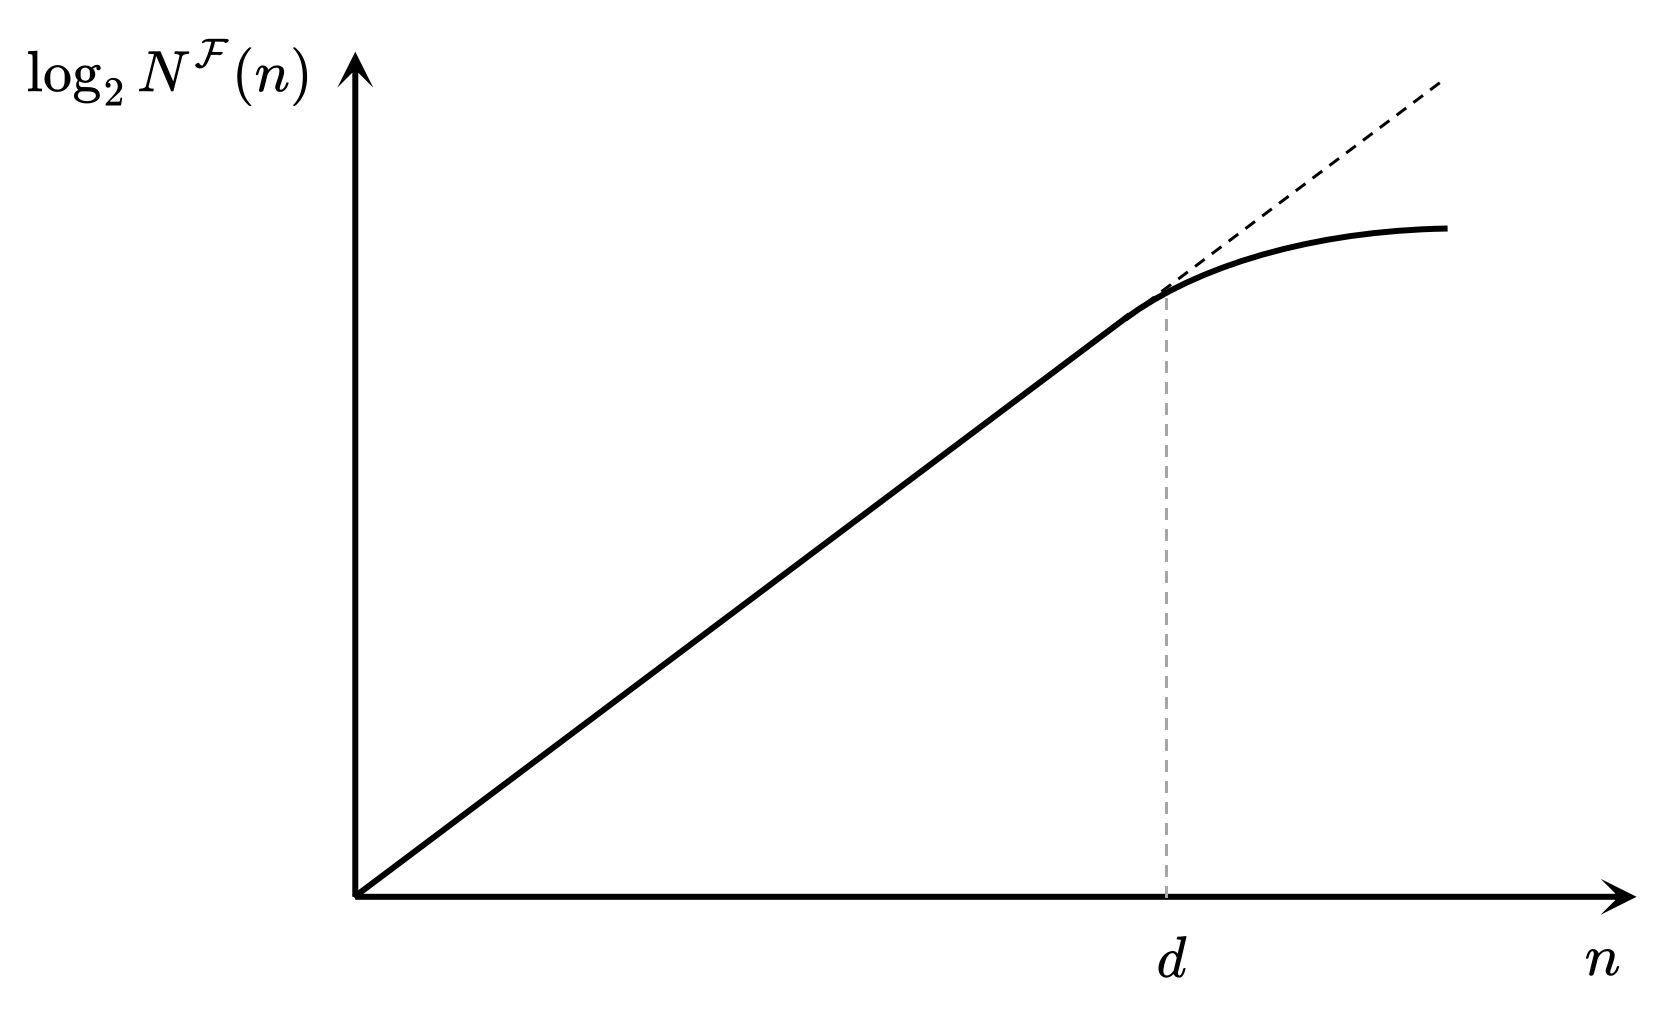
\includegraphics[width=.7\textwidth]{pic/C2_vc-dimension.png}
\end{figure} 

我们设$d$是使得$N^{\ca F}(n) = 2^n$成立的$n$的上确界. 现在想要对于$n>d$给出$N^{\ca F}(n)$的一个上界. 我们可以不妨考虑$0^{d+1}$不能被取到的情况,直接得到以下命题(至于为什么可以如此不妨假设,等待之后详细补充,现暂时留作思考)
\begin{proposition}
    对于$n > d$,有 
    \[
    N^{\ca F}(n) \le \sum_{k=0}^{d} \binom{n}{k} = \ca{O}(n^d)
    \]
\end{proposition}

下面正式给出VC维度的定义
\begin{definition} (VC维度)
    
\end{definition}